\section{Spatial Discretization Schemes}
\label{spatialdiscretization}

We discretize space with cell-centered finite volume methods (\ref{cc} ), the box method (\ref{box})
or a staggered grid scheme.
Grid adaption is available for both box and cell-centered finite volume method.
In general, the spatial  parameters, especially the porosity, have to be assigned on
the coarsest level of discretization.

\subsection{Box Method -- A Short Introduction}\label{box}

The so called box method unites the advantages of the finite-volume (FV) and
finite-element (FE) methods.

First, the model domain $\Omega$ is discretized with a FE mesh consisting of nodes
$i$ and corresponding elements $E_k$. Then, a secondary FV mesh is constructed
by connecting the midpoints and barycenters of the elements surrounding node
$i$ creating a box $B_i$ around node $i$ (see Figure \ref{pc:box}a).

\begin{figure} [ht]
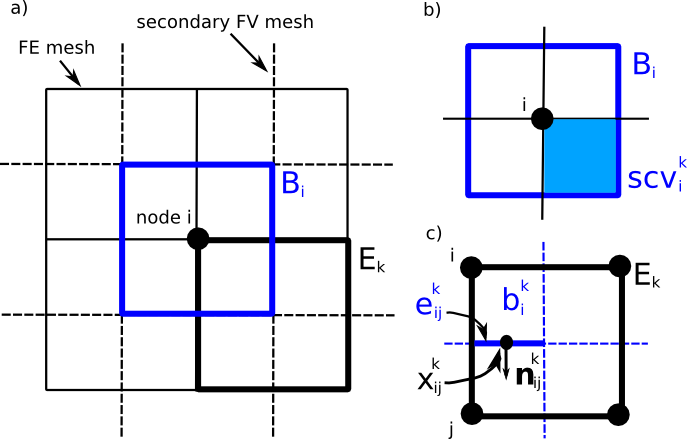
\includegraphics[width=0.8\linewidth,keepaspectratio]{png/box_disc.png}
\caption{\label{pc:box} Discretization of the box method}
\end{figure}

The FE mesh divides the box $B_i$ into subcontrolvolumes (scv's) $b^k_i$
(see Figure \ref{pc:box}b). Figure \ref{pc:box}c shows the finite element $E_k$
and the scv's $b^k_i$ inside $E_k$, which belong to four different boxes $B_i$.
Also necessary for the discretization are the faces of the subcontrolvolumes (scvf's)
$e^k_{ij}$ between the scv's $b^k_i$ and $b^k_j$, where $|e^k_{ij}|$ is the length
of the scvf. The integration points $x^k_{ij}$ on $e^k_{ij}$ and the outer normal
vector $\mathbf n^k_{ij}$ are also to be defined (see Figure \ref{pc:box}c).

The advantage of the FE method is that unstructured grids can be used, while the
FV method is mass conservative. The idea is to apply the FV method (balance of
fluxes across the interfaces) to each FV box $B_i$  and to get the fluxes across
the interfaces $e^k_{ij}$ at the integration points $x^k_{ij}$ from the FE approach.
Consequently, at each scvf the following expression results:

\begin{equation}
 	f(\tilde u(x^k_{ij})) \cdot \mathbf n^k_{ij} \: |e^k_{ij}| \qquad \textrm{with}
 	\qquad \tilde u(x^k_{ij}) = \sum_i N_i(x^k_{ij}) \cdot \hat u_i .
\end{equation}

In the following, the discretization of the balance equation is going to be derived.
From the \textsc{Reynolds} transport theorem follows the general balance equation:

\begin{equation}
	\underbrace{\int_\Omega \frac{\partial}{\partial t} \: u \, \mathrm{d}x}_{1}
	+ \underbrace{\int_{\partial\Omega} (\mathbf{v} u + \mathbf w) \cdot \textbf n \, \mathrm{d}\Gamma}_{2} = \underbrace{\int_\Omega q \, \mathrm{d}x}_{3}
\end{equation}

\begin{equation}
	f(u) = \int_\Omega \frac{\partial u}{\partial t} \, \mathrm{d}x + \int_{\Omega} \nabla \cdot
	\underbrace{\left[  \mathbf{v} u + \mathbf w(u)\right] }_{F(u)}  \, \mathrm{d}x - \int_\Omega q \, \mathrm{d}x = 0
\end{equation}
where term 1 describes the changes of entity $u$ within a control volume over
time, term 2 the advective, diffusive and dispersive fluxes over the interfaces
of the control volume and term 3 is the source and sink term. $\Omega$ denotes the
model domain and $F(u) = F(\mathbf v, p) = F(\mathbf v(x,t), p(x,t))$.

Like the FE method, the box method follows the principle of weighted residuals.
In the function $f(u)$ the unknown $u$ is approximated by discrete values at the
nodes of the FE mesh $\hat u_i$ and linear basis functions $N_i$ yielding an
approximate function $f(\tilde u)$. For $u\in \lbrace \mathbf v, p, x^\kappa \rbrace$
this means:

\begin{minipage}[b]{0.47\textwidth}
\begin{equation}
\label{eq:p}
	\tilde p = \sum_i N_i \hat{p}_i
\end{equation}
\begin{equation}
\label{eq:v}
	\tilde{\mathbf v} = \sum_i N_i \hat{\mathbf v}_i
\end{equation}
\begin{equation}
\label{eq:x}
	\tilde x^\kappa  = \sum_i N_i \hat x_i^\kappa
\end{equation}
\end{minipage}
\hfill
\begin{minipage}[b]{0.47\textwidth}
\begin{equation}
\label{eq:dp}
	\nabla \tilde p = \sum_i \nabla N_i \hat{p}_i
\end{equation}
\begin{equation}
\label{eq:dv}
	\nabla \tilde{\mathbf v} = \sum_i \nabla N_i \hat{\mathbf v}_i
\end{equation}
\begin{equation}
\label{eq:dx}
	\nabla \tilde x^\kappa  = \sum_i \nabla N_i \hat x_i^\kappa .
\end{equation}
\end{minipage}

Due to the approximation with node values and basis functions the differential
equations are not exactly fulfilled anymore but a residual $\varepsilon$ is produced.

\begin{equation}
	f(u) = 0  \qquad \Rightarrow \qquad f(\tilde u) = \varepsilon
\end{equation}

Application of the principle of weighted residuals, meaning the multiplication
of the residual $\varepsilon$ with a weighting function $W_j$  and claiming that
this product has to vanish within the whole domain,

\begin{equation}
	\int_\Omega \varepsilon W_j \, \mathrm{d}x \overset {!}{=} \: 0 \qquad \textrm{with} \qquad \sum_j W_j =1
\end{equation}
yields the following equation:

\begin{equation}
	\int_\Omega \frac{\partial \tilde u}{\partial t} W_j \, \mathrm{d}x + \int_\Omega 
	 \left[ \nabla \cdot F(\tilde u) \right] W_j  \, \mathrm{d}x - \int_\Omega q W_j \, \mathrm{d}x = \int_\Omega \varepsilon W_j \, \mathrm{d}x \: \overset {!}{=} \: 0.	
\label{eq:weightedResidual}	
\end{equation}

For standard Galerkin schemes, the weighting functions $W_j$ are chosen the same as the ansatz functions $N_j$. However, this does not yield a locally mass-conservative scheme. 
Therefore, for the Box method, the weighting functions $W_j$ are chosen as 
the piecewise constant functions over a
control volume box $B_j$, i.e.

\begin{equation}
	W_j(x) = \begin{cases}
	          1 &x \in B_j \\
		  0 &x \notin B_j.\\
	         \end{cases}
\label{eq:weightingFunctions}	         
\end{equation}
Thus, the Box method is a Petrov-Galerkin scheme, where the weighting functions do not belong to the same function space than the ansatz functions.

Inserting definition \eqref{eq:weightingFunctions} into equation \eqref{eq:weightedResidual} and using the \textsc{Green-Gaussian} integral theorem results in
\begin{equation}
	\int_{B_j} \frac{\partial \tilde u}{\partial t} \, \mathrm{d}x + \int_{\partial B_j}  F(\tilde u) \cdot \mathbf n \, \mathrm{d}\Gamma_{B_j} - \int_{B_j} q \, \mathrm{d}x  \overset {!}{=} \: 0, 	
\label{eq:BoxMassBlance}	
\end{equation}
which has to hold for every box $B_j$. 

The first term in equation \eqref{eq:BoxMassBlance} can be written as
\begin{equation}
\int_{B_j} \frac{\partial \tilde u}{\partial t} \, \mathrm{d}x = \frac{d}{dt} \int_{B_j} \sum_i \hat u_i N_i  \, \mathrm{d}x = \sum_i \frac{\partial \hat u_i}{\partial t} \int_{B_j}  N_i  \, \mathrm{d}x.
\end{equation} 
Here, a mass lumping technique is applied by assuming that the storage capacity is
reduced to the nodes. This means that the integrals $M_{i,j} = \int_{B_j}  N_i \, \mathrm{d}x$
are replaced by some mass lumped terms $M^{lump}_{i,j}$ which are defined as
\begin{equation}
	 M^{lump}_{i,j} =\begin{cases}  |B_j| &j = i\\
	0 &j \neq i,\\
	         \end{cases}
\end{equation}
where $|B_j|$ is the volume of the FV box $B_j$ associated with node $j$.
The application of this assumption yields

\begin{equation}
\label{eq:disc1}
	|B_j| \frac{\partial \hat u_j}{\partial t}
	+  \int_{\partial B_j}  F(\tilde u) \cdot \mathbf n \, \mathrm{d}\Gamma_{B_j} - Q_j = 0,
\end{equation}
where $Q_j$ is an approximation (using some quadrature rule) of the integrated source/sink term $\int_{B_j} q \, \mathrm{d}x$.

Using an implicit Euler time discretization finally
leads to the discretized form which will be applied to the mathematical
flow and transport equations:

\begin{equation}
\label{eq:discfin}
	|B_j| \frac{\hat u_j^{n+1} - \hat u_j^{n}}{\Delta t}
	+ \int_{\partial B_j}  F(\tilde u^{n+1}) \cdot \mathbf n
	\;   \mathrm{d}\Gamma_{B_j} - Q_j^{n+1} \: = 0.
\end{equation}
Equation \eqref{eq:discfin} has to be fulfilled for each box $B_j$.

\subsection{Cell Centered Finite Volume Methods -- A Short Introduction}\label{cc}
Cell-centered finite volume methods use the elements of the grid as control volumes.
For each control volume the discrete values are determined at the element/control
volume center (not required to be the barycenters). 

We consider a domain $\Omega \subset \mathbb{R}^d$, $d \in \{ 2, 3 \}$ with boundary $\Gamma = \partial \Omega$. Within this section, we consider the following elliptic problem
\begin{equation}
  \begin{aligned}
                   \nabla \cdot \left( - \mathbf{\Lambda} \nabla u \right) &= q   &&\mathrm{in} \, \Omega \\
               \left( - \mathbf{\Lambda} \nabla u \right) \cdot \mathbf{n} &= v_N &&\mathrm{on} \, \Gamma_N \\
                                                                   u &= u_D &&\mathrm{on} \, \Gamma_D.
    \label{eq:elliptic}
  \end{aligned}
\end{equation}

Here, $\mathbf{\Lambda} = \mathbf{\Lambda}(\mathbf{x}, \mathbf{u})$ is a symmetric and positive definite tensor of second rank (e.g. permeability, diffusivity, etc.), $u = u (\mathbf{x})$ is unknown and $q = q(\mathbf{x}, \mathbf{u})$ is a source/sink. 
We denote by $\mathcal{M}$ the mesh that results from the division of the domain $\Omega$ into $n_e$ control volumes $K \subset \Omega$. Each $K$ is a polygonal open set such that $K \cap L = \emptyset, \forall{K \neq L}$ and $\overline{\Omega} = \cup_{K \in \mathcal{M}} \overline{K}$. 

For the derivation of the finite-volume formulation we integrate the first equation of \eqref{eq:elliptic} over a control volume $K$ and apply the Gauss divergence theorem:

\begin{equation}
    \int_{\partial K} \left( - \mathbf{\Lambda} \nabla u \right) \cdot \mathbf{n} \, \mathrm{d} \Gamma = \int_K q \, \mathrm{d}x.
    \label{eq:ellipticIntegrated}
\end{equation}

Splitting the control volume boundary $\partial K$ into a finite number of faces $\sigma \subset \partial K$ (such that $\sigma = \overline{K} \cap \overline{L}$ for some neighboring control volume $L$) and replacing the exact fluxes by an approximation, i.e. $F_{K, \sigma} \approx \int_{\sigma} \left( - \mathbf{\Lambda}_K \nabla u \right) \cdot \mathbf{n} \mathrm{d} \Gamma$ (here $\mathbf{\Lambda}_K$ is the value of $\mathbf{\Lambda}$ associated with control volume $K$), yield
\begin{equation}
    \sum_{\sigma \subset \partial K} F_{K, \sigma} = Q_K, \quad \forall \, {K \in \mathcal{M}},
\label{eq:ccdisc}
\end{equation}
where $F_{K, \sigma}$ is the discrete flux through face $\sigma$ flowing out of cell $K$ and $Q_K := \int_K q \, \mathrm{d}x$ is the integrated source/sink term. Equation \eqref{eq:ccdisc} is the typical cell-centered finite-volume formulation. 
Finite-volume schemes differ in the way how the term 
$(\mathbf{\Lambda}_K \nabla u ) \cdot \mathbf{n} $ is approximated (i.e. the choice of the fluxes $F_{K, \sigma}$). Using the symmetry of the tensor $\mathbf{\Lambda}_K$, this term can be rewritten as 
$\nabla u  \cdot \mathbf{\Lambda}_K\mathbf{n}$, which corresponds to the directional derivative of $u$ in co-normal direction $\mathbf{\Lambda}_K\mathbf{n}$. 
In the following, the main ideas of the two-point flux approximation and the multi-point flux approximation methods are briefly described. Hereby, we restrict the discussion to the two-dimensional case.

Please also note that other types of equations, e.g. instationary parabolic problems, can be discretized by applying some time discretization scheme to the time derivatives and by using the finite-volume scheme for the flux discretization. For simplicity the discussion is restricted to the elliptic problem \eqref{eq:elliptic}.

\subsubsection{Tpfa Method}\label{cc_tpfa}
The linear two-point flux approximation is a simple but robust cell-centered finite-volume scheme, which is commonly used in commercial software. 
This scheme can be derived by using the conormal decomposition, which reads
\begin{equation}
\mathbf{\Lambda}_K \mathbf{n}_{K, \sigma} = t_{K,\sigma} \mathbf{d}_{K,\sigma} + \mathbf{d}^{\bot}_{K,\sigma}, \quad  t_{K,\sigma} = \frac{\mathbf{n}_{K, \sigma}^T \mathbf{\Lambda}_K \mathbf{d}_{K,\sigma} }{\mathbf{d}_{K,\sigma}^T \mathbf{d}_{K,\sigma}}, \; \mathbf{d}^{\bot}_{K,\sigma} = \mathbf{\Lambda}_K \mathbf{n}_{K, \sigma} - t_{K,\sigma} \mathbf{d}_{K,\sigma},
\label{eq:conormalDecTpfa}
\end{equation}
with the tensor $\mathbf{\Lambda}_K$ associated with control volume $K$, the distance vector $\mathbf{d}_{K,\sigma} := \mathbf{x}_\sigma - \mathbf{x}_K$ and $\mathbf{d}_{K,\sigma}^T \mathbf{d}^{\bot}_{K,\sigma} = 0$, see Figure \ref{pc:cctpfa} for the used notations. The same can be done for the conormal $\mathbf{\Lambda}_L \mathbf{n}_{L, \sigma}$. The $t_{K,\sigma}$ and $t_{L,\sigma}$ are the transmissibilities associated with the face $\sigma$. These transmissibilities are calculated in \Dumux by using the function \texttt{computeTpfaTransmissibility}.

\begin{figure} [ht]
\centering
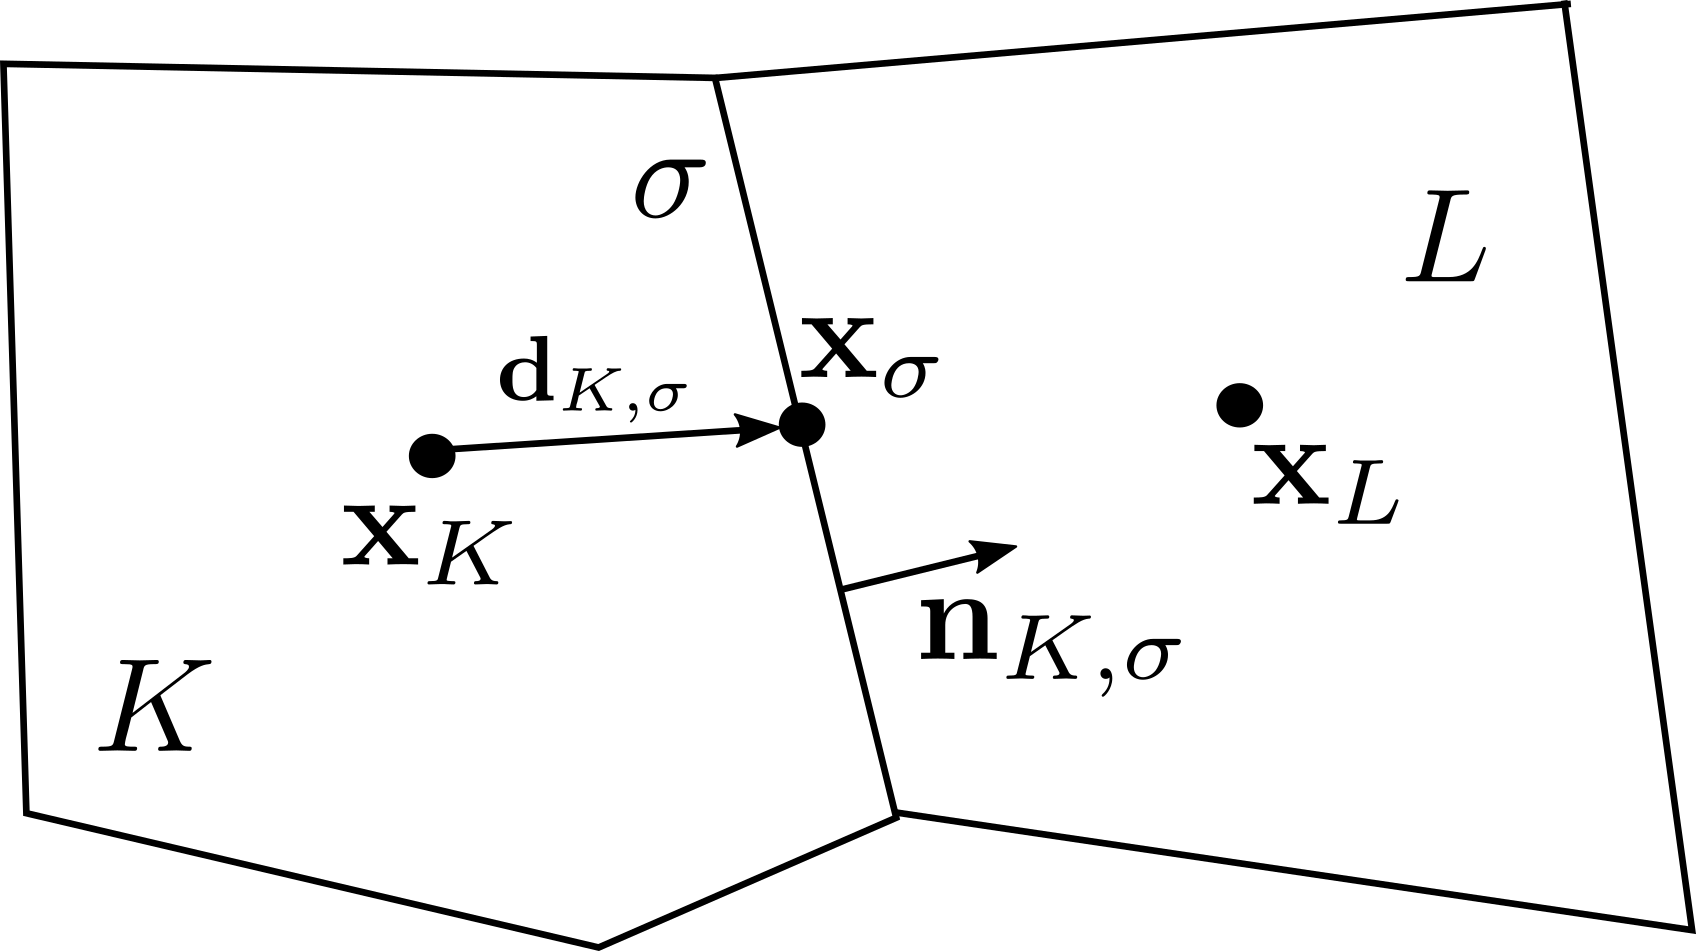
\includegraphics[width=0.4\linewidth,keepaspectratio]{png/cctpfa.png}
\caption{Two neighboring control volumes sharing the face $\sigma$.}
\label{pc:cctpfa}
\end{figure}


With these notations, it follows that for each cell $K$ and face $\sigma$ 
\begin{equation}
\nabla u \cdot \mathbf{\Lambda}_K \mathbf{n}_{K, \sigma} =  t_{K,\sigma} \nabla u \cdot \mathbf{d}_{K,\sigma} + \nabla u \cdot \mathbf{d}^{\bot}_{K,\sigma}.
\end{equation}
For the Tpfa scheme, the second part in the above equation is neglected. By using the fact that $\nabla u \cdot \mathbf{d}_{K,\sigma} \approx u_\sigma - u_K$, the discrete fluxes for face $\sigma$ are given by
\begin{equation}
F_{K,\sigma} = -\meas{\sigma}  t_{K,\sigma} (u_\sigma - u_K), \qquad F_{L,\sigma} = -\meas{\sigma}  t_{L,\sigma} (u_\sigma - u_L).
\label{eq:TPFAOneSided}
\end{equation}
Enforcing local flux conservation, i.e. $F_{K,\sigma}+F_{L,\sigma}=0$, results in 
\begin{equation}
u_\sigma = \frac{t_{K,\sigma} u_K + t_{L,\sigma} u_L}{t_{K,\sigma}  + t_{L,\sigma}}.
\end{equation}
With this, the fluxes \eqref{eq:TPFAOneSided} are rewritten as
\begin{equation}
F_{K,\sigma} = \meas{\sigma}  \frac{t_{K,\sigma} t_{L,\sigma}}{t_{K,\sigma} + t_{L,\sigma}} (u_K - u_L), \quad F_{L,\sigma} = \meas{\sigma}  \frac{t_{K,\sigma} t_{L,\sigma}}{t_{K,\sigma} + t_{L,\sigma}} (u_L - u_K).
\label{eq:TPFAFlux}
\end{equation}
By neglecting the orthogonal term, the consistency of the scheme is lost for general grids, where $\nabla u \cdot \mathbf{d}^{\bot}_{K,\sigma} \not = 0$. The consistency is achieved only for so-called K-orthogonal grids for which $\mathbf{d}^{\bot}_{K,\sigma} = 0$. For such grids we deduce that 
\begin{equation}
\frac{t_{K,\sigma} t_{L,\sigma}}{t_{K,\sigma} + t_{L,\sigma}} = \frac{\tau_{K,\sigma} \tau_{L,\sigma}}{\tau_{K,\sigma} d_{L,\sigma} + \tau_{L,\sigma} d_{K,\sigma}},
\label{eq:TPFAcoeffNew}
\end{equation}
with $\tau_{K,\sigma} := \mathbf{n}_{K, \sigma} \mathbf{\Lambda}_K\mathbf{n}_{K, \sigma}, \tau_{L,\sigma} := \mathbf{n}_{L, \sigma} \mathbf{\Lambda}_L\mathbf{n}_{L, \sigma}$, $d_{K,\sigma}:= \mathbf{n}_{K, \sigma} \cdot \mathbf{d}_{K, \sigma}$, and $d_{L,\sigma}:= \mathbf{n}_{L, \sigma} \cdot \mathbf{d}_{L, \sigma}$. This reduces, for the case of scalar permeability, to a distance weighted harmonic averaging of permeabilities.

 

\subsubsection{Mpfa Method}\label{cc_mpfa}
Expressions for the face fluxes $F_{K, \sigma}$ are obtained by introducing intermediate face unknowns $u_\sigma$ in addition to the cell unknowns $u_K$ and enforcing the physically motivated continuity of fluxes and continuity of the solution across the faces. For a face $\sigma$ between the two polygons $K$ and $L$ these conditions read:
\begin{equation}
    \begin{aligned}
        &F_{K, \sigma} + F_{L, \sigma} = 0 \\
        &{u}_{K,\sigma} = {u}_{L,\sigma} = {u}_{\sigma}.
        \label{eq:sigmaConditions}
    \end{aligned}
\end{equation}
Using these conditions, the intermediate face unknowns ${u}_\sigma$ can be eliminated and the fluxes are expressed as a function of the cell unknowns $u_N$ and associated transmissibilities $t^N_{K,\sigma}$:

\begin{equation}
    F_{K,\sigma} = \sum_{N \in \mathcal{S}_{K,\sigma}} t^N_{K,\sigma} u_{N}.
    \label{eq:FVFluxExpression}
\end{equation}

\begin{figure} [ht]
\centering
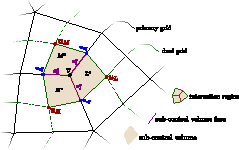
\includegraphics[width=0.8\linewidth,keepaspectratio]{pdf/mpfa_iv.pdf}
\caption{Interaction region for the Mpfa-O method. The graphic on the right illustrates how the sub-control volume $L^v$ and face $\sigma^v_2$ are embedded in cell $L$. Note that the face stencils for all sub-control volume faces in the depicted interaction region are $\mathcal{S}_{\sigma^v_i} = \{ K,L,M \}$, meaning that the fluxes over the sub-control volume faces depend on the three cell unknowns $u_K, u_L, u_M$.}
\label{pc:interactionRegion_mpfa}
\end{figure}

The main difference between the various finite-volume schemes available is the assembly of the face fluxes, i.e. the computation of the $t^N_{K,\sigma}$ and the size of $\mathcal{S}_{K,\sigma}$. For the Tpfa, that has been presented in the last section, the stencil and transmissibilities are given as
\begin{equation*}
\mathcal{S}_{K,\sigma} = \lbrace K,L \rbrace, \quad t^K_{K,\sigma} =  \meas{\sigma}  \frac{t_{K,\sigma} t_{L,\sigma}}{t_{K,\sigma} + t_{L,\sigma}},\; t^L_{K,\sigma} =  -\meas{\sigma}  \frac{t_{K,\sigma} t_{L,\sigma}}{t_{K,\sigma} + t_{L,\sigma}},
\end{equation*}
with $t_{K,\sigma},t_{L,\sigma}$ as defined in equation \eqref{eq:conormalDecTpfa}.

In the following, a multi-point flux approximation method (Mpfa-O method), which was introduced in \citet{A3:aavatsmark:2002}, is presented. The main difference to the Tpfa scheme is the fact that a consistent discrete gradient is constructed, i.e. the term $\nabla u \cdot \mathbf{d}^{\bot}_{K,\sigma}$ is not neglected.

For this scheme, a dual grid is created by connecting the barycenters of the cells with the barycenters of the faces ($d=2$) or the barycenters of the faces and edges ($d=3$). This divides each cell into sub-control volumes $K^v$. Analogously, each face is sub-divided into sub-control volume faces $\sigma^v$, see Figure \ref{pc:interactionRegion_mpfa}. We allow for piecewise constant $\mathbf{\Lambda}$ (denoted as $\mathbf{\Lambda}_K$ for each cell $K$) and construct discrete gradients $\nabla_\mathcal{D}^{K^v} u$ (per sub-control volume $K^v$). 
In the following, we restrict our discussion to the two-dimensional setup that is shown in Figure \ref{pc:interactionRegion_mpfa}.  
Here, the discrete gradients are constructed to be consistent such that the following conditions hold:
\begin{equation}
\nabla_\mathcal{D}^{K^v} u \cdot (\mathbf{x}_{\sigma^v_1}- \mathbf{x}_{K}) = u_{\sigma^v_1} - u_K, \quad \nabla_\mathcal{D}^{K^v} u \cdot (\mathbf{x}_{\sigma^v_3}- \mathbf{x}_{K}) = u_{\sigma^v_3} - u_K.
\end{equation}
Thus, a discrete gradient (for sub-control volume $K^v$) that fulfills  these conditions is given as
\begin{equation}
\nabla_\mathcal{D}^{K^v} u  = \mathbb{D}^{-T}_{K^v}
 \begin{bmatrix}
  u_{\sigma^v_1} - u_K \\
  u_{\sigma^v_3} - u_K
 \end{bmatrix}, \qquad \text{ with }\; \mathbb{D}_{K^v} := 
  \begin{bmatrix}
   \mathbf{x}_{\sigma^v_1}- \mathbf{x}_K & \mathbf{x}_{\sigma^v_3} - \mathbf{x}_K
 \end{bmatrix}.
 \label{eq:MPFAGradientRecons}
\end{equation}

This enables us to write the discrete flux across $\sigma^v_1$ from cell $K$ as follows:
\begin{equation}
    F_{K, \sigma^v_1} := - |\sigma^v_1| \mathbf{n}_{\sigma^v_1}^T \mathbf{\Lambda}_K \nabla_\mathcal{D}^{K^v} u.
    \label{eq:discreteFlux}
\end{equation}
Inserting the discrete gradient, yields
\begin{equation}
    F_{K, \sigma^v_1} = \omega_{K,\sigma^v_1\sigma^v_1}(u_K - u_{\sigma^v_1}) + \omega_{K,\sigma^v_1 \sigma^v_3}(u_K - u_{\sigma^v_3}),
    \label{eq:discreteFluxRef}
\end{equation}
with $(\omega_{K,\sigma^v_1\sigma^v_1},\omega_{K,\sigma^v_1 \sigma^v_3})^T = |\sigma^v_1| \mathbb{D}^{-1}_{K^v}\mathbf{\Lambda}_K \mathbf{n}_{\sigma^v_1}$. These values are calculated in \Dumux by using the function \texttt{computeMpfaTransmissibility}.
\\ \ \\
To deduce a cell-centered scheme, the introduced face unknowns $u_{\sigma^v_i}$ have to be eliminated. This is done by enforcing flux continuity for each sub-control volume face, i.e.
\begin{align}
F_{K, \sigma^v_1} + F_{L, \sigma^v_1} &= 0, \\ F_{K, \sigma^v_3} + F_{M, \sigma^v_3} &= 0, \\ F_{L, \sigma^v_2} + F_{M, \sigma^v_2} &= 0.
\end{align}
This results in a system of equations for the face unknowns $\mathbf{u}_{\sigma}$
\begin{equation}
\mathbb{A}^{3\times 3} \mathbf{u}_{\sigma} = \mathbb{B}^{3\times 3} \mathbf{u},
\end{equation}
where $\mathbf{u}$ contains the three cell unknowns $u_K,u_L,u_M$ and $\mathbf{u}_{\sigma}$ the three face unknowns $u_{\sigma^v_1}, u_{\sigma^v_2}, u_{\sigma^v_3}$. 
Inserting these face unknowns into the flux expression \eqref{eq:discreteFluxRef} yields
\begin{equation}
    F_{K,\sigma^v_i} = \sum_{N \in \lbrace K,L,M \rbrace } t^N_{K,\sigma^v_i} u_{N} = \mathbf{t}_{K,\sigma^v_i} \cdot \mathbf{u},
    \label{eq:FVFluxExpressionSubFace}
\end{equation}
for each cell $K$ and sub-control volume face $\sigma^v_i$. 

% \subsubsection{NLTPFA}\label{cc_nltpfa}
% TODO

\subsection{Staggered Grid -- A Short Introduction}\label{staggered}

\begin{figure}[ht]
\centering
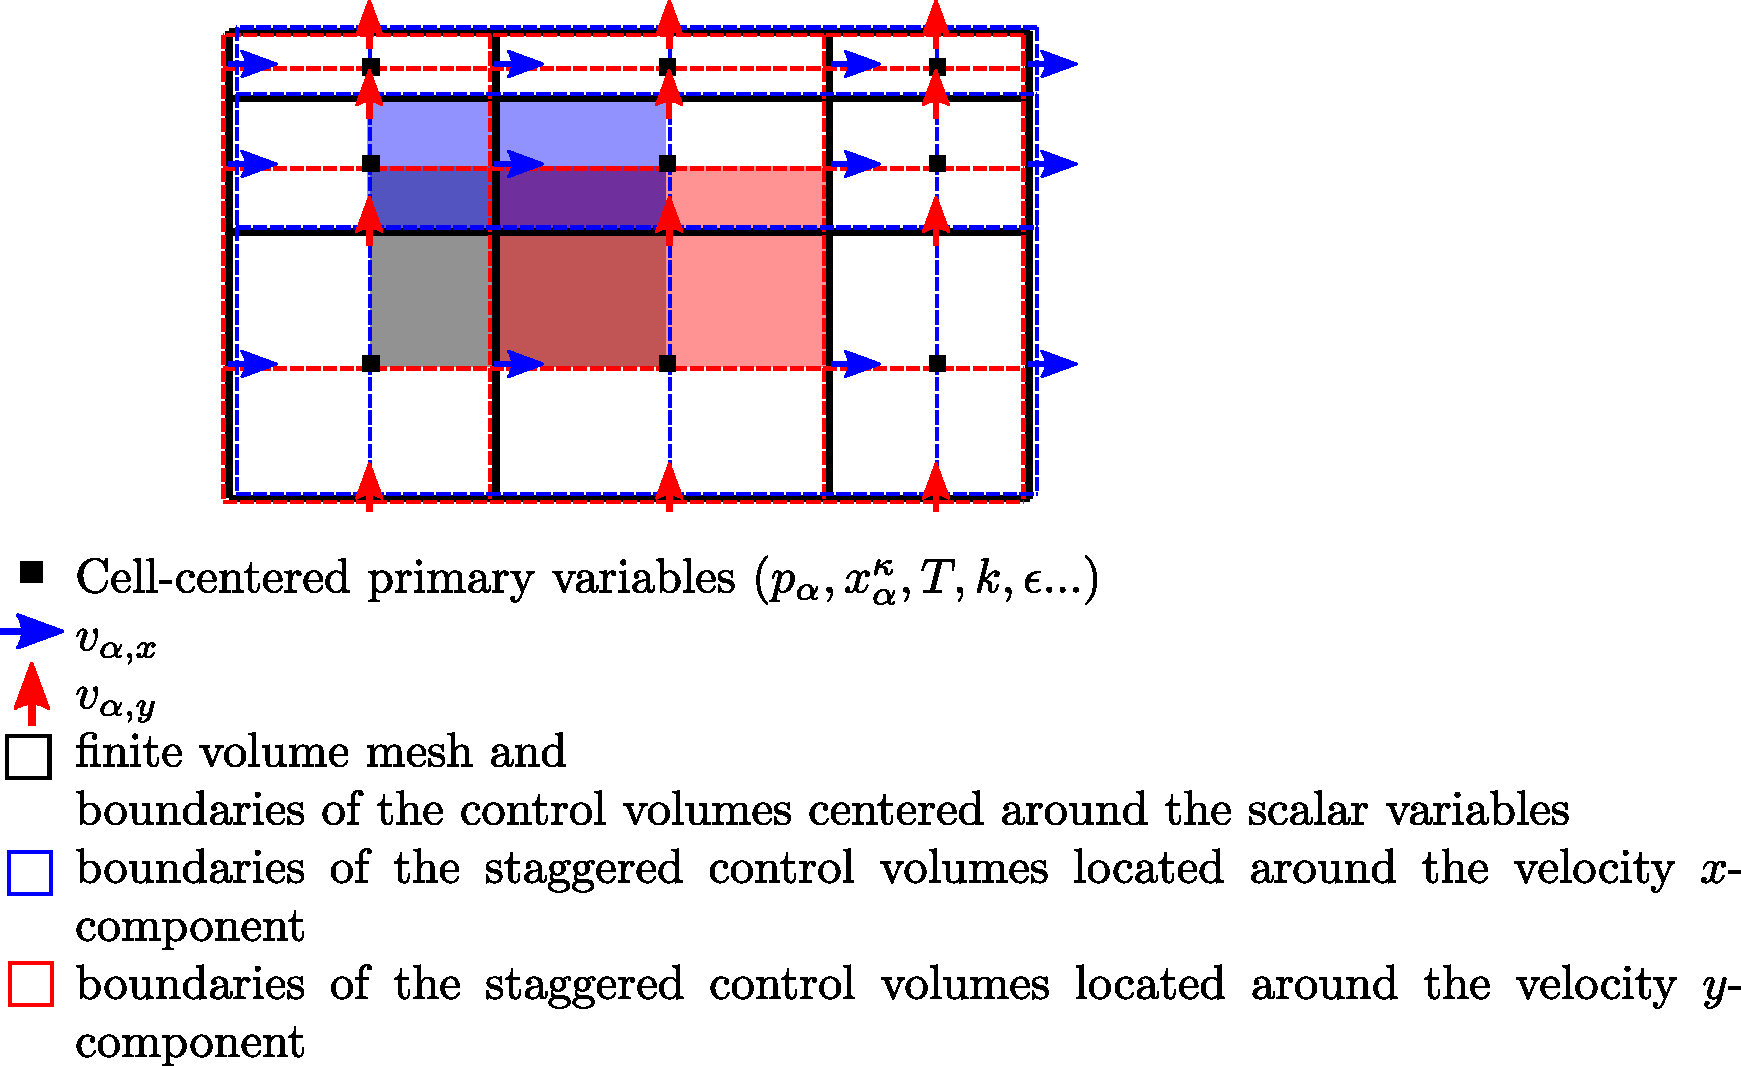
\includegraphics[width=.8\linewidth]{./pdf/staggered_grid.pdf}
\caption{\label{pc:staggered} Discretization of the staggered-grid method. The figure shows the different control volume arrangements, which are staggered with respect to each other. There are the control volumes centered around the scalar primary variables in black, the control volumes located around the $x$-component of the velocity in blue and the control volumes located around the $y$-components of the velocity in red. The control volume boundaries are given by lines. Additionally, there is one shaded example control volume each.\\
In the two-dimensional free-flow models, the continuity equation is discretized using the black control volumes, the $x$-component of the momentum equation is discretized using the blue control volumes and the $y$-component is discretized using the red control volumes. In three dimensions this works analogously.}
\end{figure}

The staggered-grid or marker-and-cell method uses a finite volume method with different control volumes for different equations. There are control volumes centered around the scalar primary variables. They correspond to the finite volume mesh. Additionally, there are control volumes located around the $x,y$ and (in 3D) $z$ velocity components which are shifted in the $x,y$ and $z$ direction, such that the velocity components are located on the edges of the cell-centered finite volume mesh (see Figure~\ref{pc:staggered}). As for the cell-centered method, the fluxes are evaluated at the edges of each control volume with a two-point flux approximation, cf. \ref{cc}.\par
The staggered-grid method is robust, mass conservative, and free of pressure oscillations
but should, as the cell-centered TPFA method, only be applied for structured grids.
Currently, all free-flow models in \Dumux use the staggered-grid discretization.
